\section{Implementering}
\subsection{Uafhængighed}


Vi benytter os ikke af andre shells i vores shell, og anser derfor vores program som værende uafhængigt. 

\subsection{Hostname}
For at udskrive hostnavnet i kommando-prompt'en, har vi åbnet filen "/proc/sys/kernel/Hostname" med fopen. Derefter læser vi første linje i filen ind i en buffer med fgets, og scanner linjen ind i vores hostname variabel med sscan. Til sidst lukker vi filen med fclose. Der er ikke noget fejlhåndtering på om filen indeholder noget, eller om den overhovedet eksisterer, med den begrundelse at vi initialiserer vores hostname variabel med strengen "DEFAULT", og derefter overskriver denne variabel, hvis altså filen eksisterer og indeholder tekst. Hvis ikke, bliver variablen ikke overskrevet, og shell'en vil altså udksrive "DEFAULT".

\subsection{Kommando håndtering}

\subsubsection{Valg af exec funktion}
Vi valgte først at afgrænse de mulige exec funktioner til de tre, der understøttede automatisk opslag efter eksekverbare filer i de filkataloger, der er specifiseret i PATH miljøvariabelen. Disse er execlp(), execvp() og execvpe(). Dette gør det let at køre kommandoer som ls og wc.

Funktion en execvpe() blev udelukket, fordi den understøtter ekstra funktionalitet, som vi ikke har brug for i form af muligheden for at specifisere miljøet af filer den eksekverede.

Forskellen på execlp() og execvp() er kun formateringen af argumenterne, og her foretrak vi execvp(), frodi vi har brugt den før.
\subsection{Baggrundskørsel af kommandoer}

\subsection{Redirection}

\subsection{Piping}
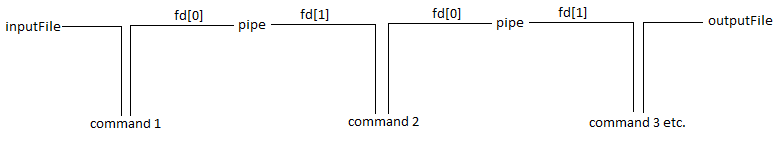
\includegraphics[width=1.1\textwidth]{pipefig}\par\vspace{1cm}

\subsection{Exit kommando}
Afslutning af bosh programmet sker, når brugeren skriver "exit" i kommandolinjen. I filen bosh.c i metoden executeshellcmd() foregår der et check af kommandoerne. Hvis den første kommando er "exit", så returner executeshellcmd() tallet 1 til den kaldende metode, main metoden. Her bliver terminate sat til 1 og while loopet, der holder bosh kørende ved at chekke om terminate IKKE er 1, vil slutte og derved også bosh.

\subsection{ctrl+c}
Vi fanger ctrl+c gennem kommandoen "signal(SIGINT, interruptRun);". Denne fanger ethvert ctrl+c og, i stedet for at interrupte bosh-kørselen, kaldes "void interruptRun(int dummy)" metoden. interrruptRun udskriver blot "caught ctrl+c" og fortsætter herefter kørslen af programmet. Grunden til at vi ikke sender interruptet videre ned i evt. kørende programmer, er at disse samtidig vil fange det samme ctrl+c input og terminere. Altså er der ikke behov at vi aktivt terminerer dem. Det skal dog også nævnes at dette ikke vil terminere evt. baggrundsprocesser, da disse ikke vil fange ctrl+c inputtet, men da vi har modelleret vores shell efter linux's indbyggede terminal, og denne har samme opførsel, så antager vi at dette er acceptabelt. 

